\documentclass[11pt,a4paper]{article}

\usepackage[margin=2.2cm]{geometry}
\usepackage{graphicx}
\usepackage{booktabs}
\usepackage{caption}
\usepackage{subcaption}
\usepackage{hyperref}
\usepackage{amsmath}
\usepackage{amssymb}
\usepackage{parskip}
\usepackage{titlesec}
\usepackage{xcolor}
\usepackage{enumitem}
\usepackage{microtype}
\usepackage{float}

\hypersetup{colorlinks=true, linkcolor=blue!60!black, urlcolor=blue!60!black}
\titlespacing*{\section}{0pt}{10pt}{4pt}
\titlespacing*{\subsection}{0pt}{7pt}{2pt}

\setlength{\parskip}{5pt}

\begin{document}

% ─── Title ──────────────────────────────────────────────────────────────────
\begin{center}
  {\LARGE\bfseries Breathe Karachi: End-to-End AQI Forecasting Pipeline}\\[6pt]
  {\large Project Report — Pearls AQI Predictor}\\[4pt]
  {\normalsize Abdullah Khan Sherwani \quad|\quad June 2026}
\end{center}

\hrule
\vspace{6pt}

% ─── Abstract ───────────────────────────────────────────────────────────────
\begin{abstract}
\noindent
Breathe Karachi is a fully serverless, end-to-end machine learning pipeline that
forecasts Karachi's US Air Quality Index (AQI) four days ahead. The system collects
raw weather and pollutant data hourly from public APIs, engineers 141 features per
day, retrains three ML models daily, and serves predictions through a Streamlit
dashboard—all without a persistent server. Three model families are trained and
evaluated — Ridge Regression, LightGBM, and LSTM — with the best-performing
model each run selected via rolling-origin cross-validation.
The live dashboard is available at \url{https://breathe-karachi.onrender.com}.
\end{abstract}

\vspace{4pt}
\hrule
\vspace{6pt}

% ─── 1. System Architecture ─────────────────────────────────────────────────
\section{System Architecture}

The pipeline is split into four loosely coupled modules, each a standalone Python
script, with MongoDB Atlas as the sole shared state store.

\begin{table}[H]
\centering
\caption{Technology stack}
\begin{tabular}{ll}
\toprule
\textbf{Layer} & \textbf{Technology} \\
\midrule
Data sources      & Open-Meteo Archive, Forecast, and Air Quality APIs \\
Feature \& model store & MongoDB Atlas (serverless) \\
Models            & Ridge Regression, LightGBM, LSTM (TensorFlow/Keras) \\
Automation        & GitHub Actions + cron-job.org \\
Explainability    & SHAP \\
Dashboard         & Streamlit + Flask (deployed on Render) \\
\bottomrule
\end{tabular}
\end{table}

\noindent Data flows as follows:
\[
\texttt{APIs} \;\xrightarrow{\text{hourly}}\; \texttt{feature\_store} \;\xrightarrow{\text{engineering}}\;
\texttt{feature\_store (processed)} \;\xrightarrow{\text{daily}}\; \texttt{model\_registry}
\;\xrightarrow{}\; \texttt{predictions}
\]

All pipeline stages authenticate to MongoDB via GitHub Secrets; no file-system
state is shared between runs.

% ─── 2. Feature Pipeline ────────────────────────────────────────────────────
\section{Feature Pipeline}

\subsection{Data Acquisition}
Historical data is fetched from two Open-Meteo endpoints: the ERA5 archive for
weather and the air quality archive for pollutants. The weather backfill extends
to 2018-01-01 (\textasciitilde3\,077 rows stored), but air quality values are
only available from August 2022 onward; rows before that date have no AQI labels.
Incremental hourly updates append only the latest day.

\subsection{Feature Engineering}
\texttt{preprocess\_daily\_data.py} applies a fixed 17-step pipeline per run,
producing \textbf{141 features} per daily row:

\begin{itemize}[noitemsep,topsep=0pt]
  \item IQR capping on 12 outlier-prone columns; log$_1$p transforms for PM$_{2.5}$ and CO
  \item Wind direction encoded as sine/cosine; stagnant-air binary flag
  \item Calendar features: month, season dummies, weekday dummies, cyclical sin/cos encodings
  \item Lag features: AQI at $t{-}1,\ldots,t{-}14$; PM$_{2.5}$, CO, NO$_2$ lags
  \item Rolling statistics: 3-, 7-, 14-day means, std, min, max; exponential weighted means
  \item Physics-inspired features: dew point, vapour pressure deficit (VPD), boundary layer height
  \item Interaction terms: PM$_{2.5}\!\times\!$Humidity, CO$\!\times\!$Temperature
  \item Weather lead features $t{+}1$ to $t{+}4$, filled from the Open-Meteo 5-day forecast for the latest rows
  \item Open-Meteo air-quality leads: AOD, dust, UV index $t{+}1$ to $t{+}4$
        (PM$_{2.5}$ leads are engineered but excluded from the production model; see Section~5.3)
\end{itemize}

The final four rows always have NaN lead features (no future observations exist).
These are filled from the Open-Meteo forecast API before upserting. Target columns
(\texttt{AQI\_t+1} through \texttt{AQI\_t+4}) remain NaN intentionally for those rows.

% ─── 3. Exploratory Data Analysis ───────────────────────────────────────────
\section{Exploratory Data Analysis}

\begin{figure}[H]
  \centering
  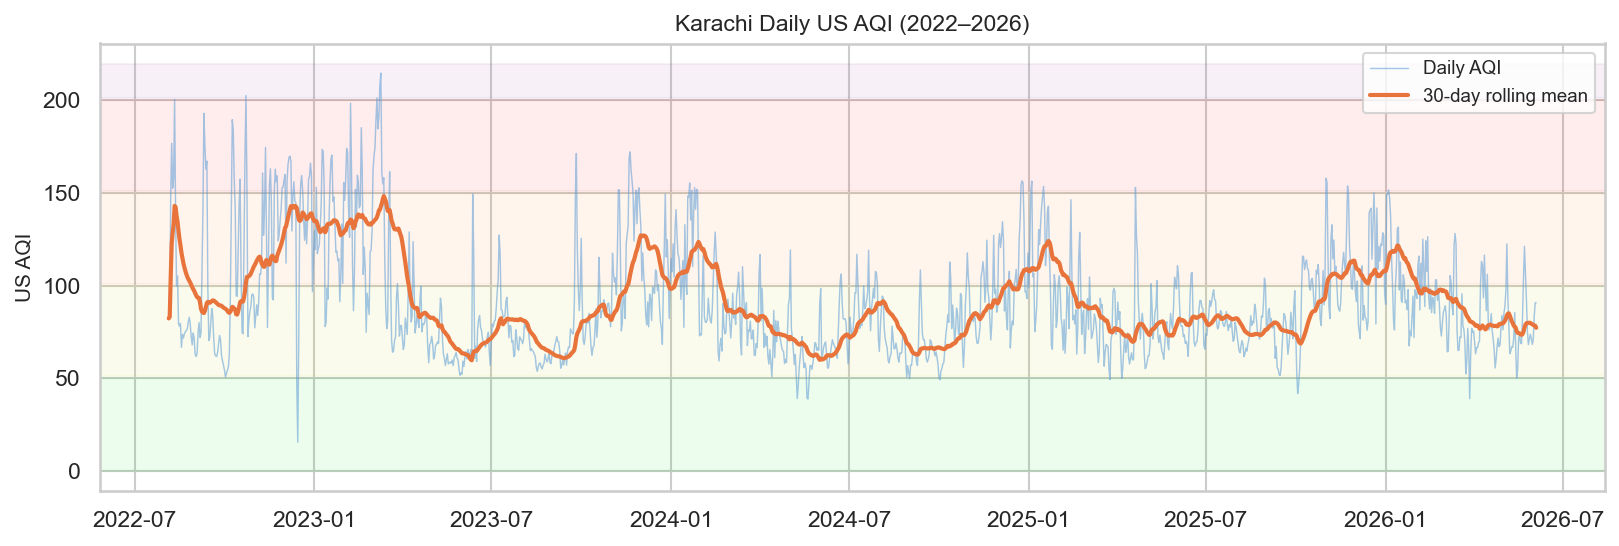
\includegraphics[width=\linewidth]{report_figures/fig_timeseries.png}
  \caption{Karachi daily US AQI (Aug 2022–Jun 2026) with 30-day rolling mean.
           Coloured bands mark EPA categories: Good (green), Moderate (yellow),
           Unhealthy for Sensitive Groups (orange), Unhealthy (red).
           Air-quality data is unavailable before Aug 2022; weather backfill
           extends to 2018. Training uses rows from 2023-01-01 onward.}
\end{figure}

\begin{figure}[H]
  \centering
  \begin{subfigure}[t]{0.56\linewidth}
    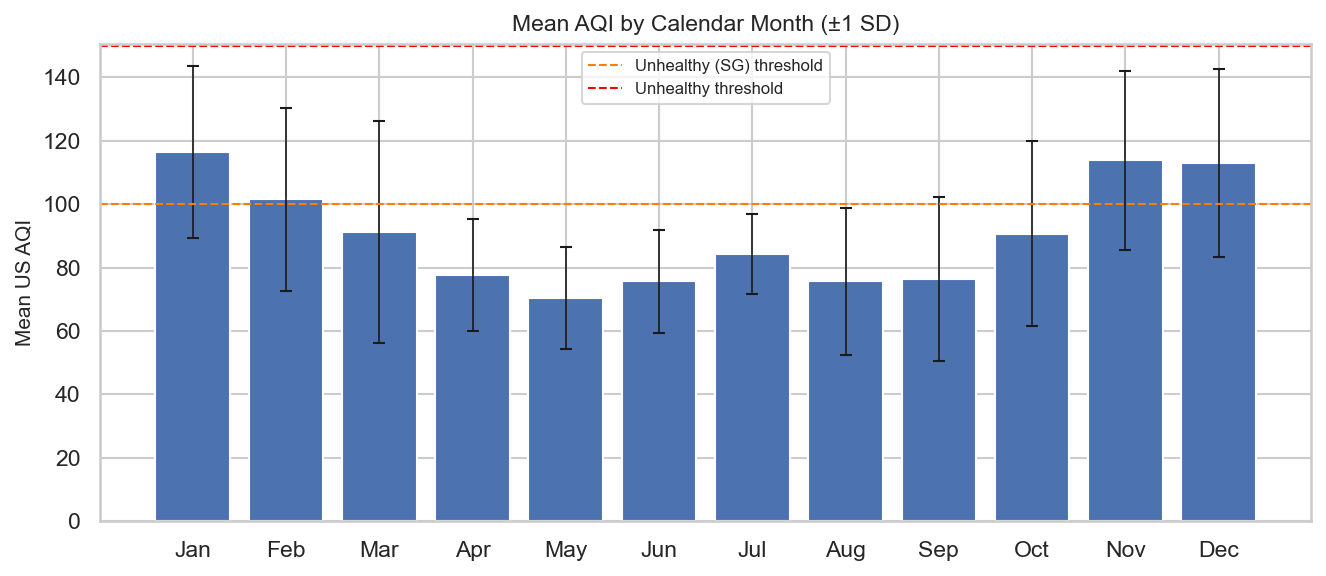
\includegraphics[width=\linewidth]{report_figures/fig_monthly_aqi.png}
    \caption{Mean AQI $\pm$1 SD by calendar month. January, November, and December
             average above 100 (Unhealthy for Sensitive Groups), driven by
             temperature inversions that trap surface pollutants.
             May is the cleanest month ($\approx$70 mean AQI).}
  \end{subfigure}
  \hfill
  \begin{subfigure}[t]{0.42\linewidth}
    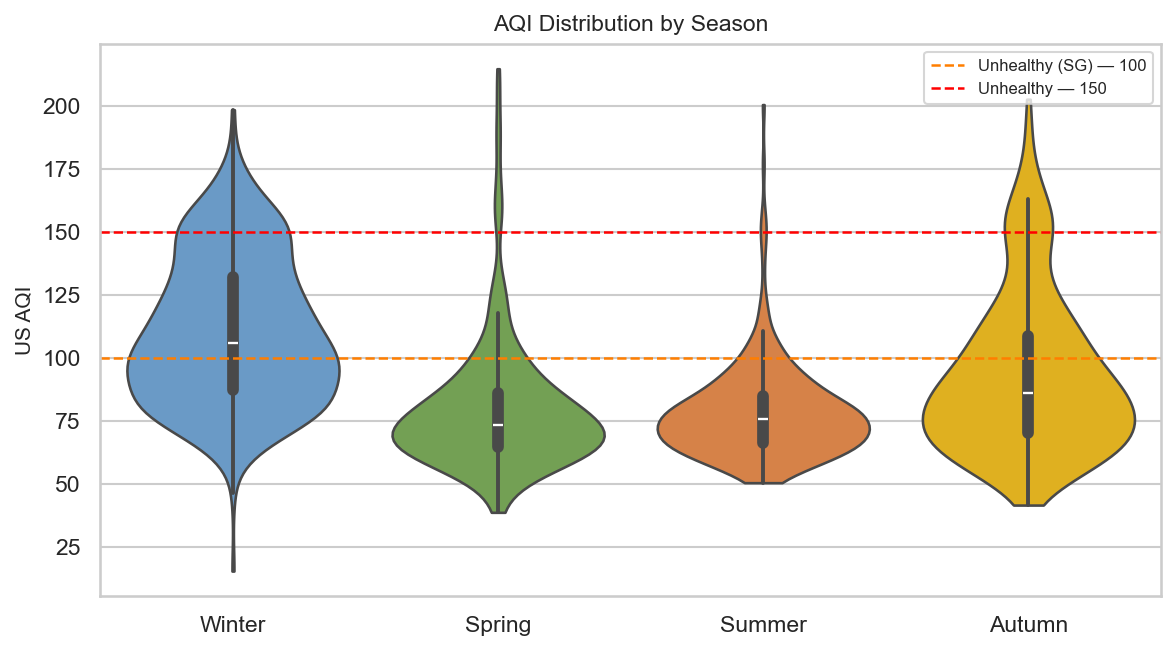
\includegraphics[width=\linewidth]{report_figures/fig_seasonal_violin.png}
    \caption{AQI distribution by meteorological season. Winter has both the
             highest median and the broadest spread, with a substantial mass
             above the Unhealthy threshold (red dash). Summer and Spring
             concentrate below 100.}
  \end{subfigure}
  \caption{Strong seasonal structure motivates month and season as engineered features.}
\end{figure}

\begin{figure}[H]
  \centering
  \begin{subfigure}[t]{0.48\linewidth}
    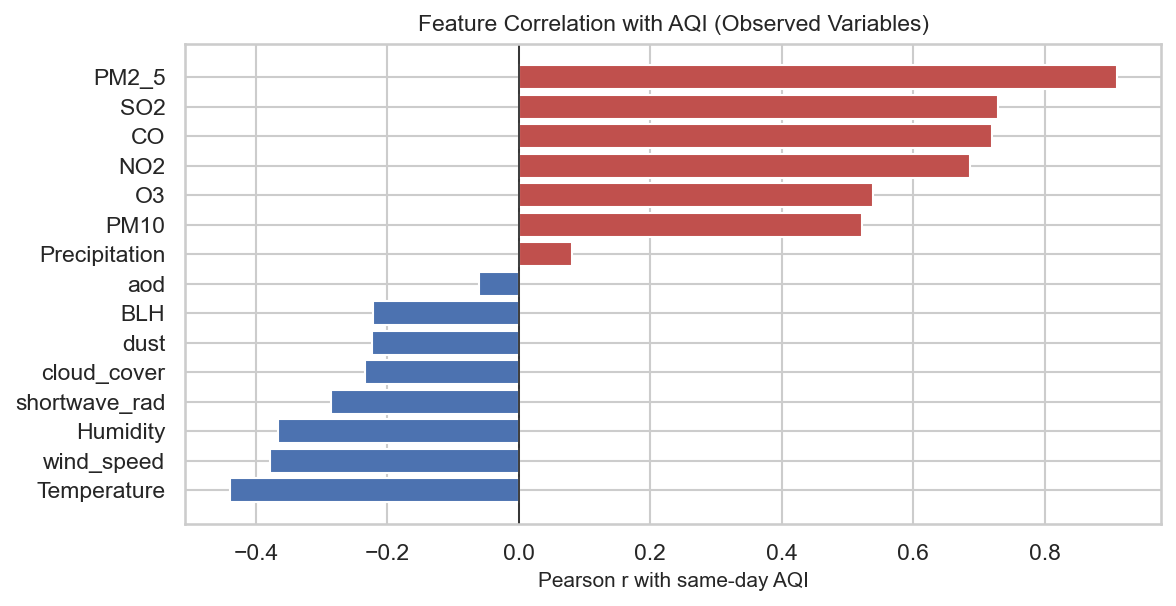
\includegraphics[width=\linewidth]{report_figures/fig_corr_aqi.png}
    \caption{Pearson $r$ of observed variables with same-day AQI.
             PM$_{2.5}$ ($r=0.91$) dominates, followed by SO$_2$, CO, and NO$_2$.
             Temperature ($r=-0.45$) and wind speed ($r=-0.41$) are the
             strongest negative predictors — higher wind disperses pollutants.}
  \end{subfigure}
  \hfill
  \begin{subfigure}[t]{0.50\linewidth}
    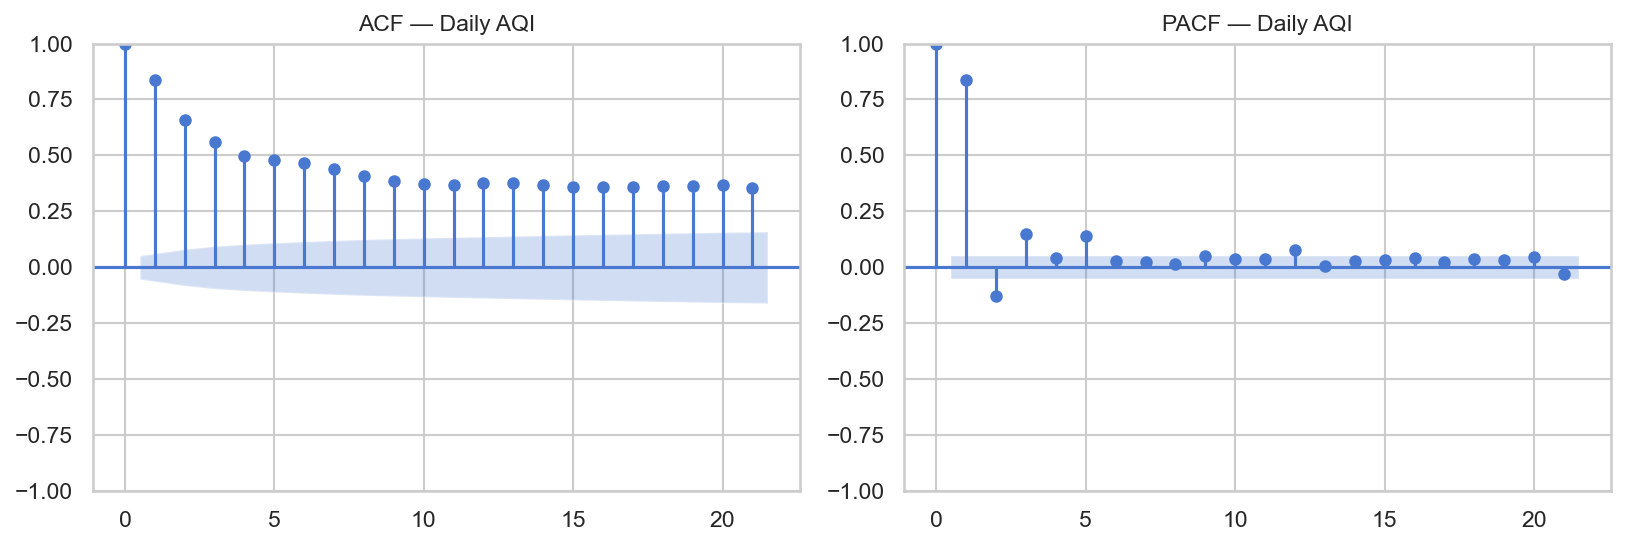
\includegraphics[width=\linewidth]{report_figures/fig_acf_pacf.png}
    \caption{ACF and PACF of the daily AQI series. ACF decays slowly
             (ACF at lag 1: 0.84, lag 3: 0.56, lag 4: 0.50), confirming
             persistent multi-day memory and motivating lag and rolling-window
             features. PACF cuts off sharply after lag 1, indicating most of
             the higher-order autocorrelation is mediated by the first lag.}
  \end{subfigure}
  \caption{Feature motivation: correlations and autocorrelation structure of the AQI series.}
\end{figure}

\textbf{SHAP feature importance.}\; All three models are explained via model-class-appropriate
SHAP methods: TreeExplainer for LightGBM, LinearExplainer for Ridge, and Expected Gradients
(GradientSHAP via \texttt{tf.GradientTape}) for LSTM. Values are persisted to MongoDB after
each training run and rendered on the dashboard.

\textit{LightGBM} (current run): PM$_{2.5}$ and its log transform dominate across all horizons,
followed by the seasonal cycle (\texttt{doy\_cos}), aerosol lead features
(\texttt{aod\_t1}--\texttt{t3}, \texttt{dust\_roll\_mean\_7}), and 14-day AQI rolling statistics.

\textit{Ridge}: the seasonal cycle (\texttt{doy\_cos}) ranks first, followed by 7--30-day
AQI/PM$_{2.5}$ rolling statistics (\texttt{PM2\_5\_ewm\_7}, \texttt{AQI\_roll\_min\_7}).
Consistent with its linear structure, Ridge relies on smoothed pollution history rather than
the most recent reading.

\textit{LSTM}: Expected-Gradients attributions highlight aerosol lead features
(\texttt{aod\_t4}, \texttt{aod\_t3}) ahead of PM$_{2.5}$ directly, suggesting the recurrent
architecture learns to exploit near-future aerosol optical depth as a forward signal.

\begin{figure}[H]
  \centering
  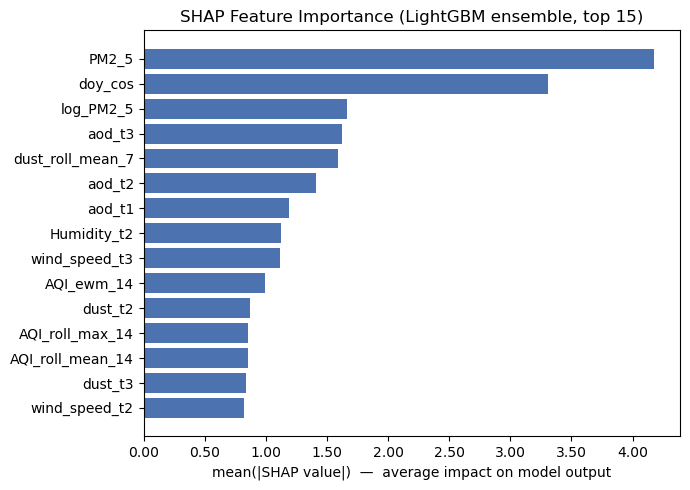
\includegraphics[width=0.78\linewidth]{report_figures/fig_shap.png}
  \caption{Mean $|\text{SHAP value}|$ for the rolling-CV-selected LightGBM (as of 2026-06-06).
           PM$_{2.5}$ and its log transform dominate; \texttt{doy\_cos} captures the
           seasonal cycle; AOD and dust lead features reflect aerosol loading at
           forecast horizons; 14-day AQI rolling statistics encode medium-term
           pollution memory.}
\end{figure}

% ─── 4. Training Pipeline ───────────────────────────────────────────────────
\section{Training Pipeline \& Models}

\texttt{train.py} follows a two-step protocol on every daily run:

\begin{enumerate}[noitemsep,topsep=2pt]
  \item \textbf{Holdout evaluation} — time-aware split (last 90 days = test).
        Each model is trained and scored per horizon (d1–d4).
  \item \textbf{Full retrain} — each model refit on all labeled rows
        (2023-01-01 to present, \textasciitilde1\,247 rows) and saved to
        \texttt{model\_registry}; old versions are purged automatically.
\end{enumerate}

A small multiplicative jitter ($\pm5\%$) is applied to lead features at training
time to bridge the train/serve gap caused by forecast error in production leads
(deterministic seed 42).

\textbf{PerHorizonWrapper (LGBM only).}\; LightGBM trains one \texttt{LGBMRegressor} per
forecast horizon, wrapped in \texttt{PerHorizonWrapper} so each sub-model fits its
horizon-specific error distribution independently. Ridge uses scikit-learn's
\texttt{MultiOutputRegressor} and LSTM uses a native Dense(4) output layer — both
produce all four horizons in a single forward pass.

\textbf{Ridge Regression.}\; StandardScaler + Ridge with $\alpha=1.0$. Used as
a fast linear baseline.

\textbf{LightGBM.}\; Per-horizon \texttt{LGBMRegressor} with L1/L2 regularization
and a two-stage early-stopping protocol: (1) discover the optimal iteration on a
15\% validation tail, (2) refit on all rows with that count scaled proportionally.
This ensures the deployed model uses every observation without risking overfitting.

\textbf{LSTM.}\; Sequence-to-4 architecture, 7-day input window, two stacked LSTM layers
(64 then 32 units, $L_2$ regularisation), dropout 0.4, Dense(4) output. Independent
scalers for inputs and targets; trained for up to 150 epochs with early stopping
(patience 25) and adaptive learning-rate reduction.

% ─── 5. Key Blockers and Fixes ──────────────────────────────────────────────
\section{Key Blockers and How They Were Fixed}

\subsection{LightGBM Severe Overfitting (10.97$\times$ train/test RMSE ratio)}

\textbf{Problem.}\; The original configuration used \texttt{n\_estimators=500},
\texttt{max\_depth=7}, \texttt{num\_leaves=63}, no regularization, and a dead
\texttt{subsample} parameter — \texttt{subsample\_freq} defaulted to 0, so bagging
never applied. The result was train R$^2\approx0.999$ and test/train RMSE ratio
of 10.97$\times$.

\textbf{Fix.}\; \texttt{lgbm\_model.py} was rewritten with the following changes:

\begin{table}[H]
\centering
\caption{LightGBM parameter changes}
\begin{tabular}{lcc}
\toprule
\textbf{Parameter} & \textbf{Before} & \textbf{After} \\
\midrule
\texttt{n\_estimators}     & 500 (fixed)   & 2000 (ceiling, early-stop) \\
\texttt{max\_depth}        & 7             & 4 \\
\texttt{num\_leaves}       & 63            & 15 \\
\texttt{subsample\_freq}   & 0 (dead)      & 1 (active) \\
\texttt{min\_child\_samples} & default     & 30 \\
\texttt{reg\_alpha}        & 0             & 0.1 \\
\texttt{reg\_lambda}       & 0             & 1.0 \\
Early stopping             & none          & 50 rounds on val tail \\
\bottomrule
\end{tabular}
\end{table}

\noindent\textbf{Result:}\; train/test RMSE ratio dropped from 10.97$\times$ to
\textbf{1.40$\times$}. LightGBM was subsequently confirmed by rolling-origin CV
as the best model across all horizons.

\subsection{Misleading 60-Day Single Holdout}

\textbf{Problem.}\; A narrow 60-day holdout (the most recent, calm-weather window)
showed Ridge winning (RMSE 10.19) with LightGBM a close second. This was a
window-selection artifact: the calm recent tail flattered linear and autoregressive
models.

\textbf{Diagnosis.}\; Multi-window holdouts (60, 90, 120, 180, 270 days) and
rolling-origin cross-validation (5-fold TimeSeriesSplit + Diebold-Mariano test)
were run. Results completely reversed the 60-day conclusion:

\begin{table}[H]
\centering
\caption{Test RMSE by holdout window (lower = better)}
\begin{tabular}{rccc}
\toprule
\textbf{Holdout days} & \textbf{Ridge} & \textbf{LGBM} & \textbf{LSTM} \\
\midrule
60  & \textbf{10.19} & 10.54 & 11.64 \\
90  & 12.73 & \textbf{11.88} & 11.10 \\
180 & 14.67 & \textbf{13.70} & 19.73 \\
270 & 16.14 & \textbf{13.71} & 17.65 \\
Rolling-origin CV & 28.03$\pm$22.34 & \textbf{16.69$\pm$4.22} & 22.96$\pm$9.69 \\
\bottomrule
\end{tabular}
\end{table}

\textbf{Fix.}\; The 60-day result was a window-selection artifact.  Broader
evaluation windows (90, 180, 270 days) and rolling-origin CV consistently
reversed this ranking, with LightGBM leading across most windows; it has
consistently been selected by rolling-origin CV in recent runs.

\subsection{PM$_{2.5}$ Lead Features and the Shadow Model}

\textbf{Observation.}\; Including PM$_{2.5}$ forecasts ($t{+}1$ to $t{+}4$) as
input features yields R$^2\approx0.91$ — unsurprising, since PM$_{2.5}$ is the
dominant AQI driver ($r=0.91$) and the model effectively depends on it almost
entirely.

\textbf{Why they are excluded from production.}\; The Open-Meteo air quality
API supplying these values is unstable: the same future date can return
materially different PM$_{2.5}$ readings depending on when the API is queried.  The offline metrics
therefore cannot be reliably reproduced in production, so PM$_{2.5}$ leads are
excluded (\texttt{EXCLUDE\_COLS} in \texttt{train.py}).

\textbf{Shadow model.}\; A separate \textit{shadow forecast}
(\texttt{scripts/predict\_pm25\_shadow.py}) trains the same model family \emph{with}
PM$_{2.5}$ leads and writes results to a separate
\texttt{predictions\_pm25} collection for ongoing research — without affecting
the live dashboard.

\subsection{NNLS Ensemble: Added, Then Retired}

\textbf{Context.}\; Before LightGBM overfitting was fixed, the 10.97$\times$ train/test RMSE
ratio made LightGBM unreliable as a standalone model. A non-negative least squares (NNLS)
ensemble blend of all three models was introduced to compensate: per-horizon weights were
fit on a held-out window, letting Ridge and LSTM down-weight the overfit LightGBM
automatically. This improved overall accuracy and was used in production.

\textbf{Problem after the fix.}\; Once LightGBM was regularised (ratio 1.40$\times$), the
ensemble became a liability. On the most recent calm-weather window the blend over-trusted
LSTM at d2–d4, widening the mean error against Open-Meteo from $\approx$2.4 AQI
(LightGBM-only) to $\approx$5.9 AQI (blend). The ensemble weights were fit on a historical
holdout that did not represent the current regime, so the blend was systematically
mis-weighted at serving time.

\textbf{Fix.}\; The ensemble was retired. A lightweight rolling-origin CV (3-fold
\texttt{TimeSeriesSplit} on the full dataset) now selects a single best model to serve
each run, falling back to LightGBM on any failure. This is implemented in
\texttt{\_rolling\_cv\_best()} in \texttt{train.py}.

\subsection{Open-Meteo API Reliability}

\textbf{Problem.}\; GitHub Actions runners intermittently experienced timeouts and
5xx errors from Open-Meteo, causing entire pipeline runs to fail.

\textbf{Fix.}\; Retry logic with exponential back-off (up to 3 attempts; 1 s and
2 s waits) was added to the preprocessing module. API timeout raised to 60 s and
max retries to 5 for the prediction step. If the forecast-fill API fails entirely,
NaN lead features are imputed at inference time using column medians from
historical rows.

\subsection{PKT Timezone Gap (00:00–05:00)}

\textbf{Problem.}\; Hourly data fetched for ``today'' in UTC returned no rows for
midnight–5 AM PKT because those hours fall on the next UTC calendar day, leaving a
5-hour gap in the daily aggregate.

\textbf{Fix.}\; The fetch end-date was switched from UTC to the PKT calendar date,
ensuring the daily average always covers a full 24 hours.

% ─── 6. Results ─────────────────────────────────────────────────────────────
\section{Results}

\subsection{Production Model (PM$_{2.5}$ Leads Excluded)}

\begin{table}[H]
\centering
\caption{90-day holdout metrics — production configuration (141 features).
         $\dagger$~Rolling-origin CV selection (3 folds, full dataset).}
\begin{tabular}{lccc}
\toprule
\textbf{Model} & \textbf{MAE} & \textbf{RMSE} & \textbf{R$^2$} \\
\midrule
Ridge                       & 9.36 & 12.68 & 0.500 \\
LSTM                        & 9.48 & 11.95 & 0.557 \\
LightGBM$^\dagger$          & \textbf{8.77} & 11.96 & 0.555 \\
\bottomrule
\end{tabular}
\end{table}

\begin{table}[H]
\centering
\caption{LightGBM per-horizon metrics (rolling-CV-selected model, 90-day holdout)}
\begin{tabular}{lccc}
\toprule
\textbf{Horizon} & \textbf{MAE} & \textbf{RMSE} & \textbf{R$^2$} \\
\midrule
d1 &  5.57 &  7.51 & 0.825 \\
d2 &  9.15 & 12.07 & 0.547 \\
d3 & 10.04 & 13.30 & 0.448 \\
d4 & 10.34 & 13.91 & 0.400 \\
\bottomrule
\end{tabular}
\end{table}

\subsection{PM$_{2.5}$ Shadow Model (Research Only)}

The shadow pipeline trains the same model family \emph{with} PM$_{2.5}$ leads
included (145 features).  Given how completely AQI depends on PM$_{2.5}$, the
metrics are strong but are driven by the API-supplied leads discussed in
Section~5.3; the shadow model is not deployed.

\begin{table}[H]
\centering
\caption{90-day holdout metrics — PM$_{2.5}$ shadow configuration (145 features, with PM$_{2.5}$ leads)}
\begin{tabular}{lccc}
\toprule
\textbf{Model} & \textbf{MAE} & \textbf{RMSE} & \textbf{R$^2$} \\
\midrule
Ridge             & 4.55 & 5.93 & 0.891 \\
LSTM              & 4.27 & 5.93 & 0.891 \\
\textbf{LightGBM} & \textbf{3.97} & \textbf{5.51} & \textbf{0.906} \\
\bottomrule
\end{tabular}
\end{table}

\begin{table}[H]
\centering
\caption{LightGBM per-horizon metrics — PM$_{2.5}$ shadow}
\begin{tabular}{lcc}
\toprule
\textbf{Horizon} & \textbf{MAE} & \textbf{R$^2$} \\
\midrule
d1 & 3.7 & 0.92 \\
d2 & 4.2 & 0.89 \\
d3 & 4.0 & 0.91 \\
d4 & 3.9 & 0.91 \\
\bottomrule
\end{tabular}
\end{table}

\noindent The shadow model's RMSE of 5.51 vs.\ the production model's 11.96
shows how completely the prediction depends on PM$_{2.5}$: excluding the
unstable API-supplied leads costs \textasciitilde6.5 RMSE units.

\subsection{Live Sanity Check vs.\ Open-Meteo}

\begin{table}[H]
\centering
\caption{Our predictions vs.\ Open-Meteo \texttt{us\_aqi} at all horizons (all dates 2026).
         d$n$ = forecast made $n$ days before the target date.
         OM: reanalysis actuals (past); live forecast snapshot (future, values may vary between fetches).
         Dashes indicate a prediction was not yet available on that anchor day.}
\footnotesize
\begin{tabular}{@{}lccccc@{}}
\toprule
\textbf{Date} & \textbf{OM} & \textbf{d1} & \textbf{d2} & \textbf{d3} & \textbf{d4} \\
\midrule
\multicolumn{6}{l}{\textit{Past (vs.\ reanalysis actuals)}} \\
05-27 & 68.1 & 71.0 & $-$ & $-$ & $-$ \\
05-28 & 70.9 & 70.7 & 69.6 & $-$ & $-$ \\
05-29 & 73.7 & 69.3 & 67.8 & 69.1 & $-$ \\
05-30 & 71.6 & 70.2 & 70.9 & 66.0 & 68.7 \\
05-31 & 68.2 & 65.3 & 68.9 & 71.1 & 66.2 \\
06-01 & 70.8 & 68.0 & 67.5 & 73.6 & 70.2 \\
\midrule
\multicolumn{6}{l}{\textit{Current forecast (anchor 06-04, vs.\ OM live forecast)}} \\
06-05 & 92.5 & 90.6 & $-$ & $-$ & $-$ \\
06-06 & 79.9 & $-$ & 82.6 & $-$ & $-$ \\
06-07 & 72.0 & $-$ & $-$ & 77.9 & $-$ \\
06-08 & 74.6 & $-$ & $-$ & $-$ & 78.6 \\
\bottomrule
\end{tabular}
\end{table}

% ─── 7. Automation ──────────────────────────────────────────────────────────
\section{Automated CI/CD Pipeline}

Two GitHub Actions workflows, both triggered by \texttt{workflow\_dispatch} from
an external cron-job.org timer (no GitHub-native cron required, avoiding cold-start
delays):

\textbf{Feature Pipeline} (every hour): fetch new daily data $\to$ fetch new hourly
data $\to$ run feature engineering.

\textbf{Training Pipeline} (daily 7:19 AM PKT, scheduled to allow Open-Meteo
values to stabilise and provide a better anchor):
train all models $\to$ generate forecast for the current day and the three days
following $\to$ generate PM$_{2.5}$ shadow forecast $\to$ generate SHAP
explanations.

MongoDB credentials are stored as GitHub Secrets. Every run starts cold from the
repository; no local state persists between runs.

% ─── 8. Dashboard & Explainability ──────────────────────────────────────────
\section{Dashboard \& Explainability}

The Streamlit dashboard reads from MongoDB at startup and displays:

\begin{itemize}[noitemsep,topsep=0pt]
  \item Next-4-day AQI forecast tiles, colour-coded to the US AQI scale
  \item Intraday hourly AQI trend chart
  \item Historical feature-store trend and EDA charts (including the monthly boxplot)
  \item AQI alert banner for any forecasted day $>150$ (Unhealthy)
\end{itemize}

% ─── 9. Limitations & Future Work ───────────────────────────────────────────
\section{Limitations \& Future Work}

\begin{itemize}[noitemsep,topsep=0pt]
  \item \textbf{Data volume.}\; \texttt{load\_data()} filters to 2023-01-01,
        using only \textasciitilde1\,247 of the \textasciitilde3\,077 rows in
        the feature store (AQ labels begin Aug 2022; records before 2023 are
        currently unused).  Learning curves show LGBM validation RMSE still
        descending — extending the window is the highest-return improvement
        available.  LSTM, which showed strong architectural promise, was largely
        unable to realise that potential on this dataset size.
  \item \textbf{Ridge regularisation.}\; $\alpha=1.0$ is under-regularised for 141
        features; RidgeCV would be a straightforward improvement.
  \item \textbf{PM$_{2.5}$ shadow.}\; If the Open-Meteo PM$_{2.5}$ forecast values
        can be shown to be sufficiently stable and accurate, including them in
        production could reduce MAE by up to 4.7 AQI units.
\end{itemize}

% ─── 10. Conclusion ─────────────────────────────────────────────────────────
\section{Conclusion}

Breathe Karachi delivers a production-grade, fully automated AQI forecasting
service for Karachi using only free-tier cloud infrastructure. The key engineering
lessons were: (1) a narrow holdout window gives dangerously wrong model rankings —
rolling-origin CV is essential for time-series evaluation; (2) LightGBM's bagging
was silently disabled by a default parameter, causing 10.97$\times$ overfitting
that was fixed with a regularised parameter set and early stopping; and (3)
PM$_{2.5}$ leads inflate offline metrics by $\sim$6.4 RMSE units, but the
Open-Meteo air quality API supplying them is unstable — values vary between
fetches — so the gain is not reliably realizable in production.  The rolling-origin-CV-selected model (LightGBM in the current run) achieves
3.6 AQI mean error against Open-Meteo forecast values — a practically useful
forecast for daily air quality planning.

\end{document}
